\subsection{The ArchSim Simulator}

\begin{frame}{The ArchSim Simulator}

\end{frame}

\begin{frame}{The ArchSim Simulator}

ArchSim is our research simulation platform. It is highly modular and configurable.

\begin{itemize}
	\item User Mode \& Full System Simulation
	\item Modular in terms of processors, devices, and platforms
	\item High speed trace system
\end{itemize}

\end{frame}

\begin{frame}{Simulation Modes}

\centering
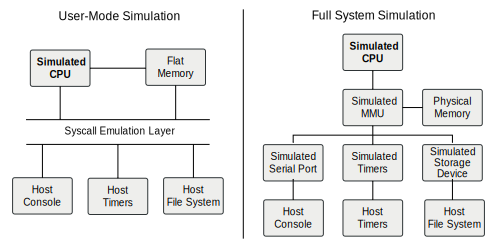
\includegraphics[width=\textwidth]{figures/user-fullsystem-compare}

\end{frame}

\begin{frame}{Modularity}

ArchSim can accept a variety of modules
\begin{itemize}
	\item GenSim processor modules
	\item External devices
\end{itemize}

This allows devices to be developed as closed-source and still used
by ArchSim

% Processor modules from GenSim
% Accepts device modules
% (Used for closed-source GPU simulation)

\end{frame}

\begin{frame}{High Speed Tracing}

\begin{minipage}[h]{0.45\textwidth}
\begin{itemize}
	\item High performance (>1MIPS)
	\item Full architectural trace
	\item Easily extensible
	\item Tools for manipulation \\\& visualisation
\end{itemize}
\end{minipage} %
\begin{minipage}[h]{0.45\textwidth}
\centering
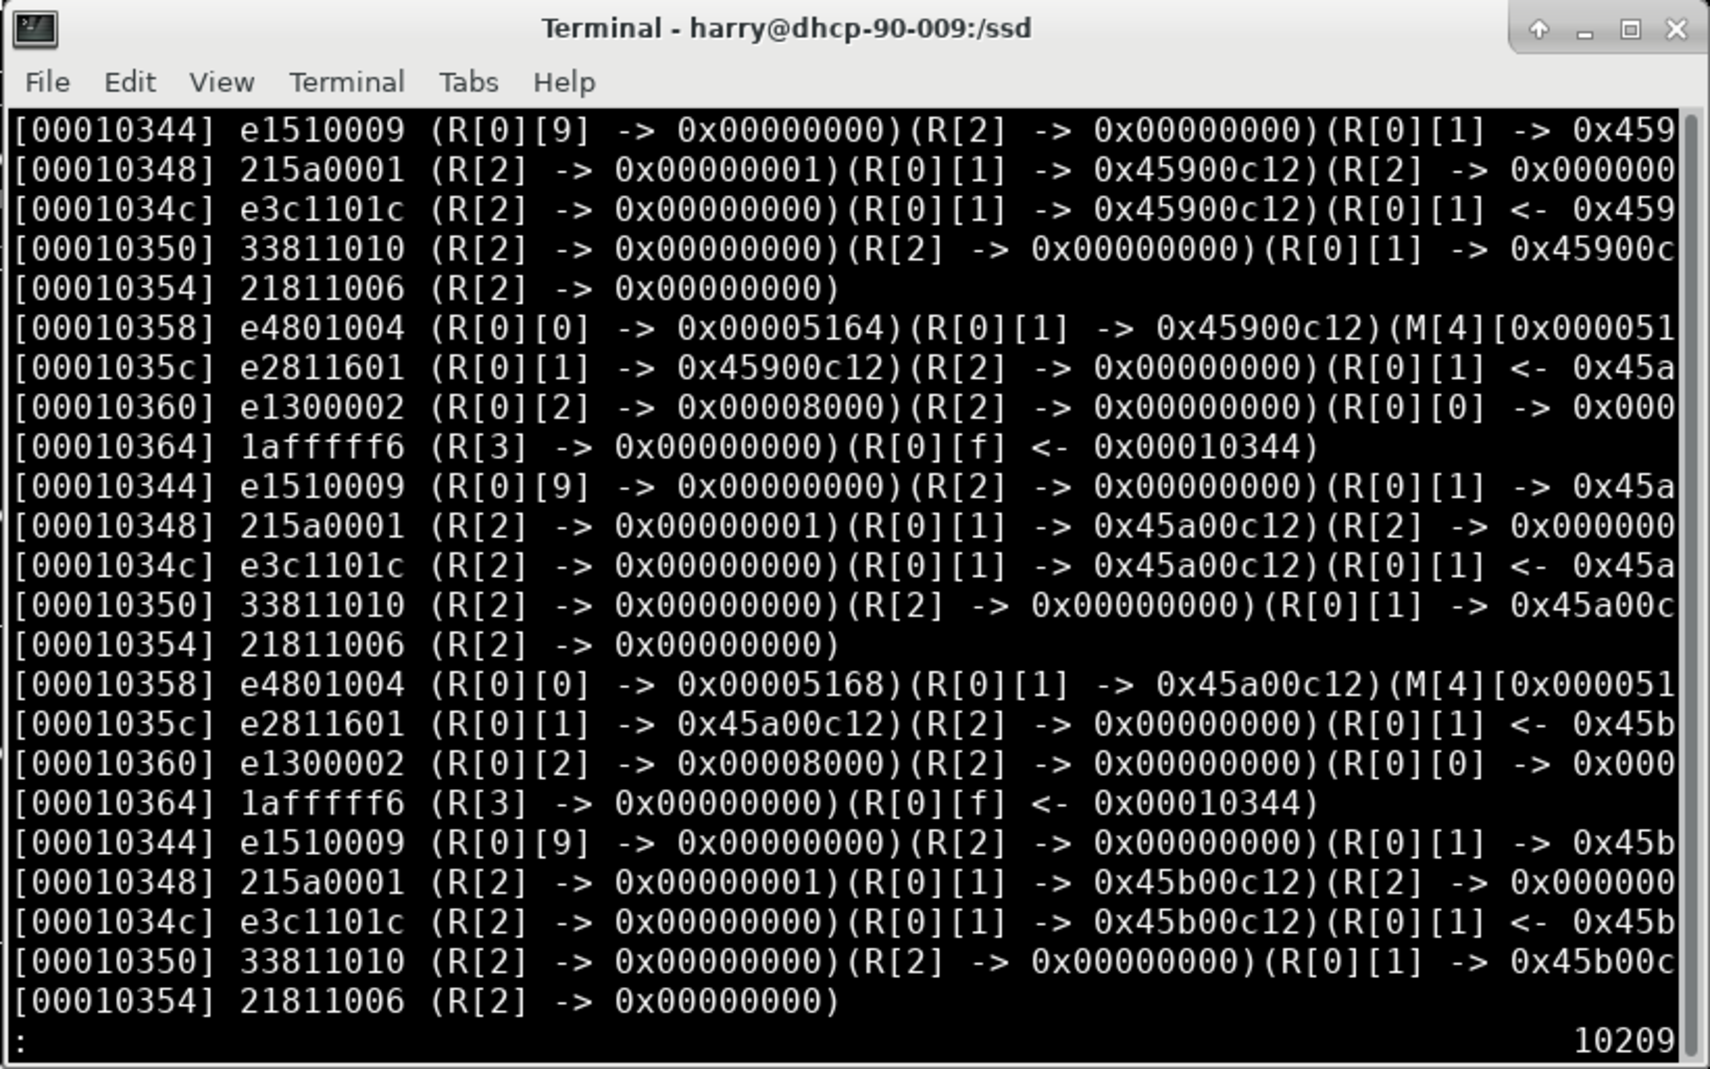
\includegraphics[width=\textwidth]{figures/trace}
\end{minipage}

\end{frame}

\begin{frame}{Short Demo}

(\url{https://www.youtube.com/watch?v=aZXx17oYumc})

\end{frame}
